\section{Visualizing Vectors: Vectors in Three Dimensions}\label{sec:geom_2}

\asyouread{
\item T/F: The viewpoint of the reader makes a difference in how vectors in 3D look.
\item T/F: If two vectors are not near each other, then they will not appear to be near each other when graphed. 
\item T/F: The parallelogram law only applies to adding vectors in 2D.
}

We ended the last section by stating we could extend the ideas of drawing 2D vectors to drawing 3D vectors. Once we understand how to properly draw these vectors, addition and subtraction is relatively easy. We'll also discuss how to find the length of a vector in 3D. 

We start with the basics of drawing a vector in 3D. Instead of having just the traditional $x$ and $y$ axes, we now add a third axis, the $z$ axis. Without any additional vectors, a generic 3D coordinate system can be seen in Figure \ref{fig:empty_3D}.

\begin{figure}[h!]
\begin{center}
\begin{tikzpicture}[x={(-.707cm,-.707cm)},y={(1cm,0cm)},z={(0,1cm)}, >=latex]

\draw [->] (0,0,0)--(3,0,0) node [below left] {$x$};
\draw [->] (0,0,0)--(0,3,0) node [right] {$y$};
\draw [->] (0,0,0)--(0,0,3) node [above] {$z$};

\foreach \x in {1,...,2}
 {\draw  (\x,-.1,0)--(\x,.1,0);
  \draw  (0,\x,-.1)--(0,\x,.1);
  \draw  (0,-.1,\x)--(0,.1,\x);
 };

\end{tikzpicture}
\end{center}
\caption{The 3D coordinate system}
\label{fig:empty_3D}
\end{figure}

In 2D, the point $(2,1)$ refers to going 2 units in the $x$ direction followed by 1 unit in the $y$ direction. In 3D, each point is referenced by 3 coordinates. The point $(4,2,3)$ is found by going 4 units in the $x$ direction, $2$ units in the $y$ direction, and 3 units in the $z$ direction. 

How does one sketch a vector on this coordinate system? As one might expect, we can sketch the vector $\vx = \bmx{c} 1\\2\\3\emx$ by drawing an arrow from the origin (the point (0,0,0)) to the point $(1,2,3)$.\footnote{Of course, we don't have to start at the origin; all that really matters is that the tip of the arrow is 1 unit in the $x$ direction, 2 units in the $y$ direction, and 3 units in the $z$ direction from the origin of the arrow.} The only ``tricky'' part comes from the fact that we are trying to represent three dimensional space on a two dimensional sheet of paper. However, it isn't really hard. We'll discover a good way of approaching this in the context of an example.\\

\example{ex_draw_3D_1}{Sketch the vectors $$\vx = \bmx{c}2\\1\\3\emx \quad \text{ and } \quad \vy = \bmx{c} 1\\3\\-1\emx$$ with their origin the origin.}
{We'll start with \vx\ first. Starting at the origin, move 2 units in the $x$ direction. This puts us at the point $(2,0,0)$ on the $x$ axis. Then, move 1 unit in the $y$ direction. (In our method of drawing, this means moving 1 unit directly to the right. Of course, we don't have a grid to follow, so we have to make a good approximation of this distance.) Finally, we move 3 units in the $z$ direction. (Again, in our drawing, this means going straight ``up'' 3 units, and we must use our best judgement in a sketch to measure this.)

This allows us to locate the point $(2,1,3)$; now we draw an arrow from the origin to this point. In Figure \ref{fig:draw_3D_vx} we have all 4 stages of this sketch. The red dotted lines show us moving down the $x$ axis in (a); in (b) we move over in the $y$ direction; in (c) we move up in the $z$ direction, and finally in (d) the arrow is drawn.

\begin{figure}[h!]
\begin{center}
\begin{tikzpicture}[x={(-.53cm,-.53cm)},y={(.75cm,0cm)},z={(0,.75cm)}, >=latex]

\begin{scope}
\draw [->] (0,0,0)--(3,0,0) node [below left] {$x$};
\draw [->] (0,0,0)--(0,3,0) node [right] {$y$};
\draw [->] (0,0,0)--(0,0,4) node [above] {$z$};

\foreach \x in {1,...,2}
 {\draw  (\x,-.1,0)--(\x,.1,0);
  };
\foreach \y in {1,...,2}
 {\draw  (0,\y,-.1)--(0,\y,.1);
  };
\foreach \z in {1,...,3}
 {\draw  (0,-.1,\z)--(0,.1,\z);
  };

\draw[dashed,red,ultra thick] (0,0,0) -- (2,0,0);
\node at (0,0,-3) {(a)};
\end{scope}

\begin{scope}[shift={(0,8,0)}]
\draw [->] (0,0,0)--(3,0,0) node [below left] {$x$};
\draw [->] (0,0,0)--(0,3,0) node [right] {$y$};
\draw [->] (0,0,0)--(0,0,4) node [above] {$z$};

\foreach \x in {1,...,2}
 {\draw  (\x,-.1,0)--(\x,.1,0);
  };
\foreach \y in {1,...,2}
 {\draw  (0,\y,-.1)--(0,\y,.1);
  };
\foreach \z in {1,...,3}
 {\draw  (0,-.1,\z)--(0,.1,\z);
  };

\draw[dashed,red,ultra thick] (0,0,0) -- (2,0,0);
\draw[dashed,red,ultra thick] (2,0,0) -- (2,1,0);

\node at (0,0,-3) {(b)};
\end{scope}

\begin{scope}[shift={(0,0,-9)}]
\draw [->] (0,0,0)--(3,0,0) node [below left] {$x$};
\draw [->] (0,0,0)--(0,3,0) node [right] {$y$};
\draw [->] (0,0,0)--(0,0,4) node [above] {$z$};

\foreach \x in {1,...,2}
 {\draw  (\x,-.1,0)--(\x,.1,0);
  };
\foreach \y in {1,...,2}
 {\draw  (0,\y,-.1)--(0,\y,.1);
  };
\foreach \z in {1,...,3}
 {\draw  (0,-.1,\z)--(0,.1,\z);
  };

\draw[dashed,red,ultra thick] (0,0,0) -- (2,0,0);
\draw[dashed,red,ultra thick] (2,0,0) -- (2,1,0);
\draw[dashed,red,ultra thick] (2,1,0) -- (2,1,3);

\filldraw [black] (2,1,3) circle (2pt);
\node at (2,1,3) [above left] {(2,1,3)};
\node at (0,0,-3) {(c)};
\end{scope}

\begin{scope}[shift={(0,8,-9)}]
\draw [->] (0,0,0)--(3,0,0) node [below left] {$x$};
\draw [->] (0,0,0)--(0,3,0) node [right] {$y$};
\draw [->] (0,0,0)--(0,0,4) node [above] {$z$};

\foreach \x in {1,...,2}
 {\draw  (\x,-.1,0)--(\x,.1,0);
  };
\foreach \y in {1,...,2}
 {\draw  (0,\y,-.1)--(0,\y,.1);
  };
\foreach \z in {1,...,3}
 {\draw  (0,-.1,\z)--(0,.1,\z);
  };

\draw[dashed,red,ultra thick] (0,0,0) -- (2,0,0);
\draw[dashed,red,ultra thick] (2,0,0) -- (2,1,0);
\draw[dashed,red,ultra thick] (2,1,0) -- (2,1,3);
\draw[thick,->] (0,0,0) -- (2,1,3);
\node at (0,0,-3) {(d)};
\end{scope}


\end{tikzpicture}
\end{center}
\caption{Stages of sketching the vector $\protect\vx$  for Example \ref{ex_draw_3D_1}.}
\label{fig:draw_3D_vx}
\end{figure}

Drawing the red lines help us find our way in our representation of three dimensional space. Without them, it is hard to see how far in each direction the vector is supposed to have gone.

To draw \vy, we follow the same procedure we used to draw \vx. We first locate the point $(1,3,-1)$, then draw the appropriate arrow. In Figure \ref{fig:draw_3D_vx_vy} we have \vy\ drawn along with \vx. We have used different colored dashed lines for each vector to help distinguish them.

Notice that this time we had to go in the negative $z$ direction; this just means we moved down one unit instead of up a unit.

\begin{figure}[h!]
\begin{center}
\begin{tikzpicture}[x={(-.53cm,-.53cm)},y={(.75cm,0cm)},z={(0,.75cm)}, >=latex]

\draw [->] (0,0,0)--(3,0,0) node [below left] {$x$};
\draw [->] (0,0,0)--(0,3,0) node [right] {$y$};
\draw [->] (0,0,-1)--(0,0,4) node [above] {$z$};

\foreach \x in {1,...,2}
 {\draw  (\x,-.1,0)--(\x,.1,0);
  };
\foreach \y in {1,...,2}
 {\draw  (0,\y,-.1)--(0,\y,.1);
  };
\foreach \z in {1,...,3}
 {\draw  (0,-.1,\z)--(0,.1,\z);
  };

\draw[dashed,red,ultra thick] (0,0,0) -- (2,0,0);
\draw[dashed,red,ultra thick] (2,0,0) -- (2,1,0);
\draw[dashed,red,ultra thick] (2,1,0) -- (2,1,3);
\draw[thick,->] (0,0,0) -- (2,1,3);

\draw[dashed,blue,ultra thick] (0,0,0) -- (1,0,0) -- (1,3,0) -- (1,3,-1);
\draw[thick,->] (0,0,0) -- (1,3,-1);

\end{tikzpicture}
\end{center}
\caption{Vectors $\protect\vx$ and $\protect\vy$ in Example \ref{ex_draw_3D_1}.}
\label{fig:draw_3D_vx_vy}
\end{figure}

} %\eexset

As in 2D, we don't usually draw the zero vector, $$\zero = \bmx{c}0\\0\\0\emx.$$ It doesn't point anywhere. It is a conceptually important vector that does not have a terribly interesting visualization.

Our method of drawing 3D objects on a flat surface -- a 2D surface -- is pretty clever. It isn't perfect, though; visually, drawing vectors with negative components (especially negative $x$ coordinates) can look a bit odd. Also, two very different vectors can point to the same place. We'll highlight this with our next two examples.\\

\example{ex_draw_3D_2}{Sketch the vector $\vx = \bmx{c} -3\\-1\\2\emx$.}
{We use the same procedure we used in Example \ref{ex_draw_3D_1}. Starting at the origin, we move in the negative $x$ direction 3 units, then 1 unit in the negative $y$ direction, and then finally up 2 units in the $z$ direction to find the point $(-3,-1,2)$. We follow by drawing an arrow. Our sketch is found in Figure \ref{fig:draw_3D_2}; \vx\ is drawn in two coordinate systems, once with the helpful dotted red lines, and once without. The second drawing makes it pretty clear that the dotted lines truly are helpful.

\begin{figure}[h!]
\begin{center}
\begin{tikzpicture}[x={(-.53cm,-.53cm)},y={(.75cm,0cm)},z={(0,.75cm)}, >=latex]

\begin{scope}
\draw [->] (-3,0,0)--(3,0,0) node [below left] {$x$};
\draw [->] (0,-1,0)--(0,3,0) node [right] {$y$};
\draw [->] (0,0,-1)--(0,0,3) node [above] {$z$};

\foreach \x in {-2,...,2}
 {\draw  (\x,-.1,0)--(\x,.1,0);
  };
\foreach \y in {1,...,2}
 {\draw  (0,\y,-.1)--(0,\y,.1);
  };
\foreach \z in {1,...,2}
 {\draw  (0,-.1,\z)--(0,.1,\z);
  };

\draw[dashed,red,ultra thick] (0,0,0) -- (-3,0,0) -- (-3,-1,0) -- (-3,-1,2);
\draw[thick,->] (0,0,0) -- (-3,-1,2);
\end{scope}

\begin{scope}[shift={(0,6,0)}]
\draw [->] (-3,0,0)--(3,0,0) node [below left] {$x$};
\draw [->] (0,-1,0)--(0,3,0) node [right] {$y$};
\draw [->] (0,0,-1)--(0,0,3) node [above] {$z$};

\foreach \x in {-2,...,2}
 {\draw  (\x,-.1,0)--(\x,.1,0);
  };
\foreach \y in {1,...,2}
 {\draw  (0,\y,-.1)--(0,\y,.1);
  };
\foreach \z in {1,...,2}
 {\draw  (0,-.1,\z)--(0,.1,\z);
  };

%\draw[dashed,red,ultra thick] (0,0,0) -- (-3,0,0) -- (-3,-1,0) -- (-3,-1,2);
\draw[thick,->] (0,0,0) -- (-3,-1,2);
\end{scope}

\end{tikzpicture}
\end{center}
\caption{Vector $\protect\vx$ in Example \ref{ex_draw_3D_2}.}
\label{fig:draw_3D_2}
\end{figure}
} %\eexset

\example{ex_draw_3D_3}{Draw the vectors $\vx = \bmx{c} 2\\4\\2\emx$ and $\vy = \bmx{c} -2\\1\\-1\emx$ on the same coordinate system.}
{We follow the steps we've taken before to sketch these vectors, shown in Figure \ref{fig:draw_3D_3}. The red dotted lines are aides for \vx\ and the blue dotted lines are aids for \vy. We again include the vectors without the dotted lines; without the lines, it is very difficult to tell which vector is which!

\begin{figure}[h!]
\begin{center}
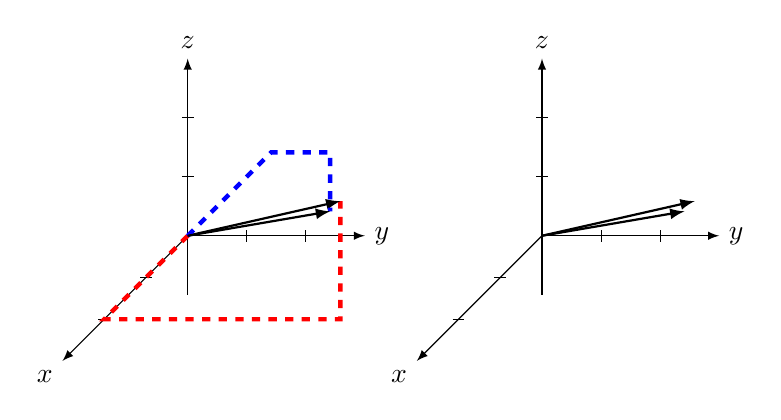
\begin{tikzpicture}[x={(-.53cm,-.53cm)},y={(.75cm,0cm)},z={(0,.75cm)}, >=latex]

\begin{scope}
\draw [->] (0,0,0)--(3,0,0) node [below left] {$x$};
\draw [->] (0,0,0)--(0,3,0) node [right] {$y$};
\draw [->] (0,0,-1)--(0,0,3) node [above] {$z$};

\foreach \x in {1,...,2}
 {\draw  (\x,-.1,0)--(\x,.1,0);
  };
\foreach \y in {1,...,2}
 {\draw  (0,\y,-.1)--(0,\y,.1);
  };
\foreach \z in {1,...,2}
 {\draw  (0,-.1,\z)--(0,.1,\z);
  };

\draw[dashed,red,ultra thick] (0,0,0) -- (2,0,0) -- (2,4,0) -- (2,4,2);
\draw[thick,->] (0,0,0) -- (2,4,2);

\draw[dashed,blue,ultra thick] (0,0,0) -- (-2,0,0) -- (-2,1,0) -- (-2,1,-1);
\draw[thick,->] (0,0,0) -- (-2,1,-1);
\end{scope}

\begin{scope}[shift={(0,6,0)}]
\draw [->] (0,0,0)--(3,0,0) node [below left] {$x$};
\draw [->] (0,0,0)--(0,3,0) node [right] {$y$};
\draw [->] (0,0,-1)--(0,0,3) node [above] {$z$};

\foreach \x in {1,...,2}
 {\draw  (\x,-.1,0)--(\x,.1,0);
  };
\foreach \y in {1,...,2}
 {\draw  (0,\y,-.1)--(0,\y,.1);
  };
\foreach \z in {1,...,2}
 {\draw  (0,-.1,\z)--(0,.1,\z);
  };

%\draw[dashed,red,ultra thick] (0,0,0) -- (1,0,0) -- (1,2,0) -- (1,2,2);
\draw[thick,->] (0,0,0) -- (2,4,2);

%\draw[dashed,blue,ultra thick] (0,0,0) -- (2,0,0) -- (2,3,0) -- (2,3,-1);
\draw[thick,->] (0,0,0) -- (-2,1,-1);
\end{scope}

\end{tikzpicture}
\end{center}
\caption{Vectors $\protect\vx$ and $\protect\vy$ in Example \ref{ex_draw_3D_3}.}
\label{fig:draw_3D_3}
\end{figure}
} %\eexset

Our three examples have demonstrated that we have a pretty clever, albeit imperfect, method for drawing 3D vectors. The vectors in Example \ref{ex_draw_3D_3} look similar because of our \textit{viewpoint}. In Figure \ref{fig:viewpoint_1} (a), we have rotated the coordinate axes, giving the vectors a different appearance. (Vector \vx\ now looks like it lies on the $y$ axis.) 

Another important factor in how things look is the scale we use for the $x$, $y$, and $z$ axes. In 2D, it is easy to make the scale uniform for both axes; in 3D, it can be a bit tricky to make the scale the same on the axes that are ``slanted.'' Figure \ref{fig:viewpoint_1} (b) again shows the same 2 vectors found in Example \ref{ex_draw_3D_3}, but this time the scale of the $x$ axis is a bit different. The end result is that again the vectors appear a bit different than they did before.
These facts do not necessarily pose a big problem; we must merely be aware of these facts and not make judgments about 3D objects based on one 2D image.\footnote{The human brain uses both eyes to convey 3D, or depth, information. With one eye closed (or missing), we can have a very hard time with ``depth perception.'' Two objects that are far apart can seem very close together. A simple example of this problem is this: close one eye, and place your index finger about a foot above this text, directly above this \textbf{WORD}. See if you were correct by dropping your finger straight down. Did you actually hit the proper spot? Try it again with both eyes, and you should see a noticable difference in your accuracy.

Looking at 3D objects on paper is a bit like viewing the world with one eye closed.}

\begin{figure}[h!]
\begin{center}
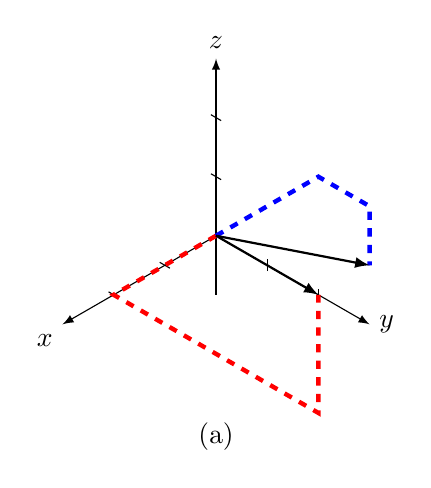
\begin{tikzpicture}[x={(-.65cm,-.375cm)},y={(.65cm,-.375cm)},z={(0,.75cm)}, >=latex]
\draw [->] (0,0,0)--(3,0,0) node [below left] {$x$};
\draw [->] (0,0,0)--(0,3,0) node [right] {$y$};
\draw [->] (0,0,-1)--(0,0,3) node [above] {$z$};
\foreach \x in {1,...,2}
 {\draw  (\x,-.1,0)--(\x,.1,0);
  };
\foreach \y in {1,...,2}
 {\draw  (0,\y,-.1)--(0,\y,.1);
  };
\foreach \z in {1,...,2}
 {\draw  (0,-.1,\z)--(0,.1,\z);
  };
\draw[dashed,red,ultra thick] (0,0,0) -- (2,0,0) -- (2,4,0) -- (2,4,2);
\draw[thick,->] (0,0,0) -- (2,4,2);
\draw[dashed,blue,ultra thick] (0,0,0) -- (-2,0,0) -- (-2,1,0) -- (-2,1,-1);
\draw[thick,->] (0,0,0) -- (-2,1,-1);
\node at (0,0,-3) [below] {(a)};
\end{tikzpicture} $\quad$ 
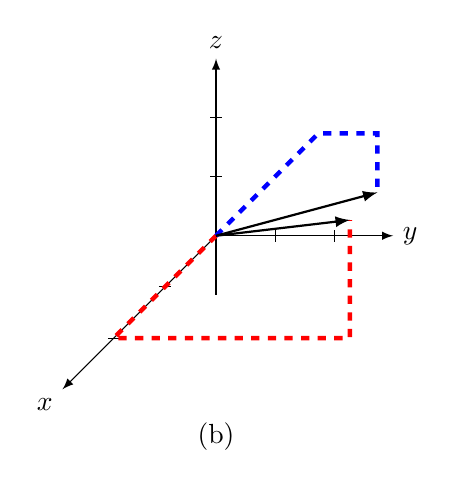
\begin{tikzpicture}[x={(-.65cm,-.65cm)},y={(.75cm,0cm)},z={(0,.75cm)}, >=latex]
\draw [->] (0,0,0)--(3,0,0) node [below left] {$x$};
\draw [->] (0,0,0)--(0,3,0) node [right] {$y$};
\draw [->] (0,0,-1)--(0,0,3) node [above] {$z$};
\foreach \x in {1,...,2}
 {\draw  (\x,-.1,0)--(\x,.1,0);
  };
\foreach \y in {1,...,2}
 {\draw  (0,\y,-.1)--(0,\y,.1);
  };
\foreach \z in {1,...,2}
 {\draw  (0,-.1,\z)--(0,.1,\z);
  };
\draw[dashed,red,ultra thick] (0,0,0) -- (2,0,0) -- (2,4,0) -- (2,4,2);
\draw[thick,->] (0,0,0) -- (2,4,2);
\draw[dashed,blue,ultra thick] (0,0,0) -- (-2,0,0) -- (-2,1,0) -- (-2,1,-1);
\draw[thick,->] (0,0,0) -- (-2,1,-1);
\node at (0,0,-3) [below] {(b)};
\end{tikzpicture}
\end{center}
\caption{Vectors $\protect\vx$ and $\protect\vy$ in Example \ref{ex_draw_3D_3} with a different viewpoint (a) and $x$ axis scale (b).}
\label{fig:viewpoint_1}
\end{figure}

We now investigate properties of vector arithmetic: what happens (i.e., how do we draw) when we add 3D vectors and multiply by a scalar? How do we compute the length of a 3D vector? \\

\noindent \large \textsf{\textbf{Vector Addition and Subtraction}} \normalsize\\

In 2D, we saw that we could add vectors together graphically using the Parallelogram Law. Does the same apply for adding vectors in 3D? We investigate in an example.\\

\example{ex_add_3D}{Let $\vx = \bmx{c}2\\1\\3\emx$ and $\vy = \bmx{c}1\\3\\-1\emx$. Sketch $\vx + \vy$. }
{We sketched each of these vectors previously in Example \ref{ex_draw_3D_1}. We sketch them, along with $\vx+\vy = \bmx{c} 3\\4\\2\emx$, in Figure \ref{fig:add_3D} (a). (We use purple dotted lines for $\vx+\vy$, which seems appropriate.)

Does the Parallelogram Law still hold? In  Figure \ref{fig:add_3D} (b), we draw additional representations of \vx\ and \vy\ to form a parallelogram (without all the dotted lines), which seems to affirm the fact that the Parallelogram Law does indeed hold.

\begin{figure}[h!]
\begin{center}
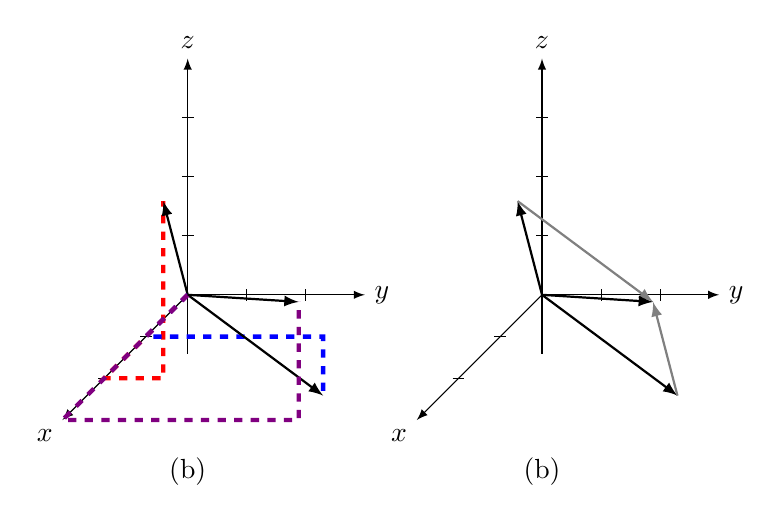
\begin{tikzpicture}[x={(-.53cm,-.53cm)},y={(.75cm,0cm)},z={(0,.75cm)}, >=latex]

\begin{scope}
\draw [->] (0,0,0)--(3,0,0) node [below left] {$x$};
\draw [->] (0,0,0)--(0,3,0) node [right] {$y$};
\draw [->] (0,0,-1)--(0,0,4) node [above] {$z$};

\foreach \x in {1,...,2}
 {\draw  (\x,-.1,0)--(\x,.1,0);
  };
\foreach \y in {1,...,2}
 {\draw  (0,\y,-.1)--(0,\y,.1);
  };
\foreach \z in {1,...,3}
 {\draw  (0,-.1,\z)--(0,.1,\z);
  };

\draw[dashed,red,ultra thick] (0,0,0) -- (2,0,0) -- (2,1,0) -- (2,1,3);
\draw[thick,->] (0,0,0) -- (2,1,3);

\draw[dashed,blue,ultra thick] (0,0,0) -- (1,0,0) -- (1,3,0) -- (1,3,-1);
\draw[thick,->] (0,0,0) -- (1,3,-1);

\draw[dashed,violet,ultra thick] (0,0,0) -- (3,0,0) -- (3,4,0) -- (3,4,2);
\draw[thick,->] (0,0,0) -- (3,4,2);

\node at (0,0,-3) {(b)};
\end{scope}

\begin{scope}[shift={(0,6,0)}]
\draw [->] (0,0,0)--(3,0,0) node [below left] {$x$};
\draw [->] (0,0,0)--(0,3,0) node [right] {$y$};
\draw [->] (0,0,-1)--(0,0,4) node [above] {$z$};

\foreach \x in {1,...,2}
 {\draw  (\x,-.1,0)--(\x,.1,0);
  };
\foreach \y in {1,...,2}
 {\draw  (0,\y,-.1)--(0,\y,.1);
  };
\foreach \z in {1,...,3}
 {\draw  (0,-.1,\z)--(0,.1,\z);
  };


\draw[thick,->] (0,0,0) -- (2,1,3);
\draw[thick,->] (0,0,0) -- (1,3,-1);
\draw[thick,->,gray] (2,1,3) -- (3,4,2);
\draw[thick,->,gray] (1,3,-1) -- (3,4,2);
\draw[thick,->] (0,0,0) -- (3,4,2);

\node at (0,0,-3) {(b)};
\end{scope}

\end{tikzpicture}
\end{center}
\caption{Vectors $\protect\vx$, $\protect\vy$, and $\protect\vx + \protect\vy$ Example \ref{ex_add_3D}.}
\label{fig:add_3D}
\end{figure}
} %\eexset

We also learned that in 2D, we could subtract vectors by drawing a vector from the tip of one vector to the other.\footnote{Recall that it is important which vector we used for the origin and which was used for the tip.} Does this also work in 3D? We'll investigate again with an example, using the familiar vectors \vx\ and \vy\ from before.\\

\example{ex_draw_3D_4}{Let $\vx = \bmx{c}2\\1\\3\emx$ and $\vy = \bmx{c}1\\3\\-1\emx$. Sketch $\vx - \vy$. }
{It is simple to compute that $\vx-\vy = \bmx{c} 1\\-2\\4\emx$. All three of these vectors are sketched in Figure \ref{fig:draw_3D_4} (a), where again \vx\ is guided by the red, \vy\ by the blue, and $\vx-\vy$ by the purple dotted lines. 

Does the 2D subtraction rule still hold? That is, can we draw $\vx - \vy$ by drawing an arrow from the tip of \vy\ to the tip of \vx? In Figure \ref{fig:draw_3D_4} (b), we translate the drawing of $\vx-\vy$ to the tip of \vy, and sure enough, it looks like it works. (And in fact, it really does.)

\begin{figure}[h!]
\begin{center}
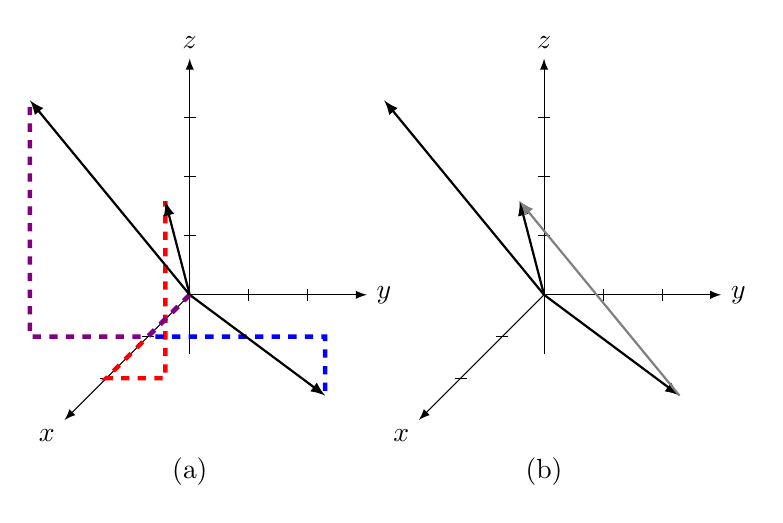
\begin{tikzpicture}[x={(-.53cm,-.53cm)},y={(.75cm,0cm)},z={(0,.75cm)}, >=latex]

\begin{scope}
\draw [->] (0,0,0)--(3,0,0) node [below left] {$x$};
\draw [->] (0,0,0)--(0,3,0) node [right] {$y$};
\draw [->] (0,0,-1)--(0,0,4) node [above] {$z$};

\foreach \x in {1,...,2}
 {\draw  (\x,-.1,0)--(\x,.1,0);
  };
\foreach \y in {1,...,2}
 {\draw  (0,\y,-.1)--(0,\y,.1);
  };
\foreach \z in {1,...,3}
 {\draw  (0,-.1,\z)--(0,.1,\z);
  };

\draw[dashed,red,ultra thick] (0,0,0) -- (2,0,0) -- (2,1,0) -- (2,1,3);
\draw[thick,->] (0,0,0) -- (2,1,3);

\draw[dashed,blue,ultra thick] (0,0,0) -- (1,0,0) -- (1,3,0) -- (1,3,-1);
\draw[thick,->] (0,0,0) -- (1,3,-1);

\draw[dashed,violet,ultra thick] (0,0,0) -- (1,0,0) -- (1,-2,0) -- (1,-2,4);
\draw[thick,->] (0,0,0) -- (1,-2,4);

\node at (0,0,-3) {(a)};
\end{scope}

\begin{scope}[shift={(0,6,0)}]
\draw [->] (0,0,0)--(3,0,0) node [below left] {$x$};
\draw [->] (0,0,0)--(0,3,0) node [right] {$y$};
\draw [->] (0,0,-1)--(0,0,4) node [above] {$z$};

\foreach \x in {1,...,2}
 {\draw  (\x,-.1,0)--(\x,.1,0);
  };
\foreach \y in {1,...,2}
 {\draw  (0,\y,-.1)--(0,\y,.1);
  };
\foreach \z in {1,...,3}
 {\draw  (0,-.1,\z)--(0,.1,\z);
  };


\draw[thick,->] (0,0,0) -- (2,1,3);
\draw[thick,->] (0,0,0) -- (1,3,-1);
\draw[thick,->,gray] (1,3,-1) -- (2,1,3);

\draw[thick,->] (0,0,0) -- (1,-2,4);

\node at (0,0,-3) {(b)};
\end{scope}

\end{tikzpicture}
\end{center}
\caption{Vectors $\protect\vx$, $\protect\vy$, and $\protect\vx - \protect\vy$ from Example \ref{ex_draw_3D_4}.}
\label{fig:draw_3D_4}
\end{figure}
} %\eexset

The previous two examples highlight the fact that even in 3D, we can sketch vectors without explicitly knowing what they are. We practice this one more time in the following example.\\

\example{ex_draw_3D_5}{Vectors \vx\ and \vy\ are drawn in Figure \ref{fig:draw_3D_5a}. Using this drawing, sketch the vectors $\vx+\vy$ and $\vx-\vy$. 
\begin{figure}[h!]
\begin{center}
\begin{tikzpicture}[x={(-.53cm,-.53cm)},y={(.75cm,0cm)},z={(0,.75cm)}, >=latex]


\draw [->] (0,0,0)--(3,0,0) node [below left] {$x$};
\draw [->] (0,0,0)--(0,3,0) node [right] {$y$};
\draw [->] (0,0,0)--(0,0,3) node [above] {$z$};

\foreach \x in {1,...,2}
 {\draw  (\x,-.1,0)--(\x,.1,0);
  };
\foreach \y in {1,...,2}
 {\draw  (0,\y,-.1)--(0,\y,.1);
  };
\foreach \z in {1,...,2}
 {\draw  (0,-.1,\z)--(0,.1,\z);
  };


\draw[thick,->] (0,0,0) -- (0,-2,1) node [above] {\vx};

\draw[thick,->] (0,0,0) -- (2,2,2)  node [above] {\vy};


\end{tikzpicture}
\end{center}
\caption{Vectors $\protect\vx$ and $\protect\vy$ for Example \ref{ex_draw_3D_5}.}
\label{fig:draw_3D_5a}
\end{figure}

}
{Using the Parallelogram Law, we draw $\vx+\vy$ by first drawing a gray version of \vy\ coming from the tip of \vx; $\vx+\vy$ is drawn in red in Figure \ref{fig:draw_3D_5b}.

To draw $\vx-\vy$, we draw a blue arrow from the tip of \vy to the tip of \vx. 

\begin{figure}[h!]
\begin{center}
\begin{tikzpicture}[x={(-.53cm,-.53cm)},y={(.75cm,0cm)},z={(0,.75cm)}, >=latex]


\draw [->] (0,0,0)--(3,0,0) node [below left] {$x$};
\draw [->] (0,0,0)--(0,3,0) node [right] {$y$};
\draw [->] (0,0,0)--(0,0,3) node [above] {$z$};

\foreach \x in {1,...,2}
 {\draw  (\x,-.1,0)--(\x,.1,0);
  };
\foreach \y in {1,...,2}
 {\draw  (0,\y,-.1)--(0,\y,.1);
  };
\foreach \z in {1,...,2}
 {\draw  (0,-.1,\z)--(0,.1,\z);
  };


\draw[thick,->] (0,0,0) -- (0,-2,1);

\draw[thick,->] (0,0,0) -- (2,2,2);

\draw[thick,->,gray] (0,-2,1) -- (2,0,3);

\draw[thick,->,red] (0,0,0) -- (2,0,3);

\draw[thick,->,blue] (2,2,2) -- (0,-2,1);

\end{tikzpicture}
\end{center}
\caption{Vectors $\protect\vx$, $\protect\vy$, $\protect\vx + \protect\vy$ and $\protect\vx - \protect\vy$ for Example \ref{ex_draw_3D_5}.}
\label{fig:draw_3D_5b}
\end{figure}
} % \eexset

\noindent \large \textsf{\textbf{Scalar Multiplication}} \normalsize\\

Given a vector \vx\ in 3D, what does the vector 2\vx\ look like? How about $-\vx$? After learning about vector addition and subtraction in 3D, we are probably gaining confidence in working in 3D and are tempted to say that 2\vx\ is a vector twice as long as \vx, pointing in the same direction, and $-\vx$ is a vector of the same length as \vx, pointing in the opposite direction. We would be right. We demonstrate this in the following example.\\

\example{ex_3D_scalar_1}{Sketch \vx, 2\vx, and $-\vx$, where $$\vx = \bmx{c} 1\\2\\3\emx.$$}
{\begin{figure}[h!]
\begin{center}
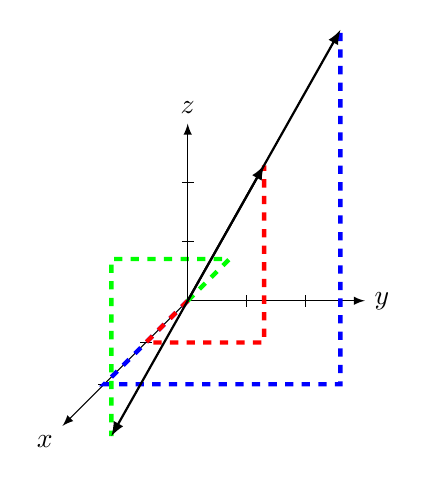
\begin{tikzpicture}[x={(-.53cm,-.53cm)},y={(.75cm,0cm)},z={(0,.75cm)}, >=latex]

\draw [->] (0,0,0)--(3,0,0) node [below left] {$x$};
\draw [->] (0,0,0)--(0,3,0) node [right] {$y$};


\foreach \x in {1,...,2}
 {\draw  (\x,-.1,0)--(\x,.1,0);
  };
\foreach \y in {1,...,2}
 {\draw  (0,\y,-.1)--(0,\y,.1);
  };
\foreach \z in {1,...,2}
 {\draw  (0,-.1,\z)--(0,.1,\z);
  };

\draw[dashed,blue,ultra thick] (0,0,0) -- (2,0,0) -- (2,4,0) -- (2,4,6);


\draw[dashed,red,ultra thick] (0,0,0) -- (1,0,0) -- (1,2,0) -- (1,2,3);


\draw[dashed,green,ultra thick] (0,0,0) -- (-1,0,0) -- (-1,-2,0) -- (-1,-2,-3);
\draw[thick,->] (0,0,0) -- (-1,-2,-3);

\draw[thick,->] (0,0,0) -- (2,4,6);
\draw[thick,->] (0,0,0) -- (1,2,3);
\draw [->] (0,0,0)--(0,0,3) node [above] {$z$};

\end{tikzpicture}
\end{center}
\caption{Sketching scalar multiples of $\protect \vx$ in Example \ref{ex_3D_scalar_1}.}
\label{fig:3D_scalar_1}
\end{figure}

It is easy to compute $$2\vx = \bmx{c}2\\4\\6\emx \quad \text{ and } \quad -\vx = \bmx{c} -1\\-2\\-3\emx.$$ These are drawn in Figure \ref{fig:3D_scalar_1}. This figure is, in many ways, a mess, with all the dotted lines. They are useful though. Use them to see how each vector was formed, and note that 2\vx\ at least looks twice as long as \vx, and it looks like $-\vx$ points in the opposite direction.\footnote{Our previous work showed that looks can be deceiving, but it is indeed true in this case.} }\\ %\eexset


\noindent \large \textsf{\textbf{Vector Length}} \normalsize\\

How do we measure the length of a vector in 3D? In 2D, we were able to answer this question by using the Pythagorean Theorem. Does the Pythagorean Theorem apply in 3D? In a sense, it does. 

Consider the vector $\vx = \bmx{c} 1\\2\\3\emx$, as drawn in Figure \ref{fig:3D_vect_length} (a), with guiding red dotted lines. Now look at part (b) of the same figure. Note how two lengths of the dotted lines have now been drawn green, and another blue dotted line has been added. 

\begin{figure}[h!]
\begin{center}
\begin{tikzpicture}[x={(-.53cm,-.53cm)},y={(.75cm,0cm)},z={(0,.75cm)}, >=latex]

\begin{scope}
\draw [->] (0,0,0)--(3,0,0) node [below left] {$x$};
\draw [->] (0,0,0)--(0,3,0) node [right] {$y$};
\draw [->] (0,0,0)--(0,0,3) node [above] {$z$};

\foreach \x in {1,...,2}
 {\draw  (\x,-.1,0)--(\x,.1,0);
  };
\foreach \y in {1,...,2}
 {\draw  (0,\y,-.1)--(0,\y,.1);
  };
\foreach \z in {1,...,2}
 {\draw  (0,-.1,\z)--(0,.1,\z);
  };

\draw[dashed,red,ultra thick] (0,0,0) -- (1,0,0) -- (1,2,0) -- (1,2,3);
\draw[thick,->] (0,0,0) -- (1,2,3);


\node at (0,0,-3) {(a)};
\end{scope}

\begin{scope}[shift={(0,6,0)}]
\draw [->] (0,0,0)--(3,0,0) node [below left] {$x$};
\draw [->] (0,0,0)--(0,3,0) node [right] {$y$};
\draw [->] (0,0,0)--(0,0,3) node [above] {$z$};

\foreach \x in {1,...,2}
 {\draw  (\x,-.1,0)--(\x,.1,0);
  };
\foreach \y in {1,...,2}
 {\draw  (0,\y,-.1)--(0,\y,.1);
  };
\foreach \z in {1,...,2}
 {\draw  (0,-.1,\z)--(0,.1,\z);
  };


\draw[dashed,green,ultra thick] (0,0,0) -- (1,0,0) -- (1,2,0);
\draw[dashed,blue,ultra thick] (0,0,0) -- (1,2,0);
\draw[dashed,red,ultra thick]  (1,2,0) -- (1,2,3);

\draw[thick,->] (0,0,0) -- (1,2,3);


\node at (0,0,-3) {(b)};
\end{scope}

\end{tikzpicture}
\end{center}
\caption{Computing the length of $\protect \vx$}
\label{fig:3D_vect_length}
\end{figure}

These green and blue dotted lines form a right triangle with the blue line forming the hyptenuse. We can find the length of the blue line using the Pythagorean Theorem. 

$$\text{length of the blue line} = \sqrt{ \text{sum of the squares of the green line lengths}}$$

That is, the length of the blue line = $\sqrt{1^2 + 2^2} = \sqrt{5}$.

Now consider this: the vector \vx\ is the hypotenuse of another right triangle: the one formed by the blue dotted line and the vertical red line. Again, we employ the Pythagorean Theorem to find its length.

$$\text{length of } \vx = \sqrt{ \text{(length of blue line)}^2 + \text{(length of red line)}^2}$$

Thus, the length of \vx\ is (recall, we denote the length of \vx\ with $||\vx||$):

\begin{align*}
||\vx|| &= \sqrt{\text{(length of blue line)}^2 + \text{(length of red line)}^2} \\
				&= \sqrt{ \sqrt{5}^2 + 3^2}\\
				&= \sqrt{ 5 + 3^2}\\
\end{align*}

Let's stop for a moment and think: where did this 5 come from in the previous equation? It came from finding the length of the blue line -- it came from $1^2+2^2$. Let's substitute that into the previous equation:

\begin{align*}
||\vx||	&= \sqrt{5+ 3^2} \\
				&= \sqrt{1^2+2^2+3^2}\\
				&= \sqrt{14}\\
\end{align*}

The key comes from the middle equation: $||\vx|| = \sqrt{1^2+2^2+3^2}$. Do those numbers 1, 2, and 3 look familiar? They are the component values of \vx! This is very similar to the definition of the length of a 2D vector. After formally defining this, we'll practice with an example.

\definition{def:3D_length}{\textbf{3D Vector Length}\\

Let $$\vx = \bmx{c}x_1\\x_2\\x_3\emx.$$ The \textit{length} of \vx, denoted $||\vx||$, is $$||\vx|| = \sqrt{x_1^2+x_2^2+x_3^2}.$$}

\example{ex_3D_vect_length}{Find the lengths of vectors \vx\ and \vy, where $$\vx = \bmx{c} 2\\-3\\5\emx \quad \text{ and } \quad \vy = \bmx{c} -4\\7\\0\emx.$$}
{We apply Definition \ref{def:3D_length} to each vector:

\begin{align*}
||\vx|| 	&= \sqrt{2^2 + (-3)^2 + 5^2} \\
					&= \sqrt{4 + 9 + 25}\\
					&= \sqrt{38}\\
\\
||\vy|| &= \sqrt{(-4)^2 + 7^2 + 0^2}\\
				&= \sqrt{16+49}\\
				&= \sqrt{65}
\end{align*}
\ } \\ %\eexset

Here we end our investigation into the world of graphing vectors. Extensions into graphing 4D vectors and beyond \textit{can} be done, but they truly are confusing on not really done except for abstract purposes. 

There are further things to explore, though. Just as in 2D, we can transform 3D space by matrix multiplication. Doing this properly -- rotating, stretching, shearing, etc. -- allows one to manipulate 3D space and create incredible computer graphics. \\

%Our investigation into the world of visualizing vectors is almost complete. We have explored vector addition, subtraction, and scalar multiplication (which also led us to the idea of measuring vector lengths). There is one final element of matrix arithmetic to explore: matrix -- vector multiplication. If \tta\ is an $n\times n$ matrix and \vx\ is an $n\times 1$ vector, we know that \tta\vx\ is also an $n\times 1$ vector. What can we learn by visualizing \vx\ and \tta\vx? In the next section, we will find out.\\

\printexercises{exercises/05_02_exercises}